\documentclass{standalone}
\usepackage{tikz}
\usetikzlibrary{arrows.meta, positioning, fit,calc}

\begin{document}
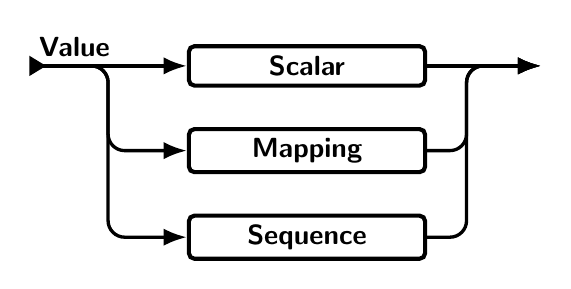
\begin{tikzpicture}[
  incoming/.style={line width=1.2pt, {Triangle[reversed]}-{Latex}},
  normal/.style={line width=1.2pt, -{Latex}},
  box/.style={
    draw,
    line width=1.5pt,
    rectangle,
    rounded corners=2pt,
    minimum width=3cm,
    minimum height=0.5cm,
    align=center,
    font=\sffamily\bfseries
  }
]

  \coordinate (start);
  \coordinate (end) at ($(start)+(6.5cm,0)$);

  % label placed north-east of the coordinate
  \node[anchor=south west] at (start) {\sffamily \bfseries Value};

  % next node
  \node[box, right=2cm of start] (scalar) {Scalar};
  \draw[incoming] (start) -- (scalar);
  \draw[normal] (scalar) -- (end);

  \node[box, below=0.5cm of scalar] (mapping) {Mapping};
  \draw[normal,rounded corners=6pt] ($(start)+(0.5cm,0)$) -- ++(0.5cm,0) |- (mapping.west);
  \draw[normal,rounded corners=6pt] ($(mapping.east)$) -- ++(0.5cm,0) |- (end);

  \node[box, below=0.5cm of mapping] (sequence) {Sequence};
  \draw[normal,rounded corners=6pt] ($(start)+(0.5cm,0)$) -- ++(0.5cm,0) |- (sequence.west);
  \draw[normal,rounded corners=6pt] ($(sequence.east)$) -- ++(0.5cm,0) |- (end);



\end{tikzpicture}
\end{document}
